


\begin{frame}{Towards a Model of Cortical Function \sof{1}{2}}


\twocol{0.52}{
\justifying

\vspace{0.5em}
The cortex of mammals has a distinct, low-level structure consisting of six 
horizontal layers that are vertically connected by local groups of about 80 to 
100 neurons forming so-called {\bf minicolumns}.

\vspace{1em}
Based on our previous efforts to model the behaviour of entorhinal grid cells 
we argue in ~\cite{Kerdels2018} that a single {\bf cortical column} can function
as an independent, {\bf autoassociative memory cell} (AMC) that utilizes a 
sparse distributed encoding.

\vspace{1em}
In~\cite{Kerdels2019b} we develop our ideas further and argue that {\bf cortical 
memory is a distributed, dynamic process} that is an intrinsic part of the 
cortical network both structurally and functionally.

}{0.4}{
\begin{figure}
\vspace{2em}
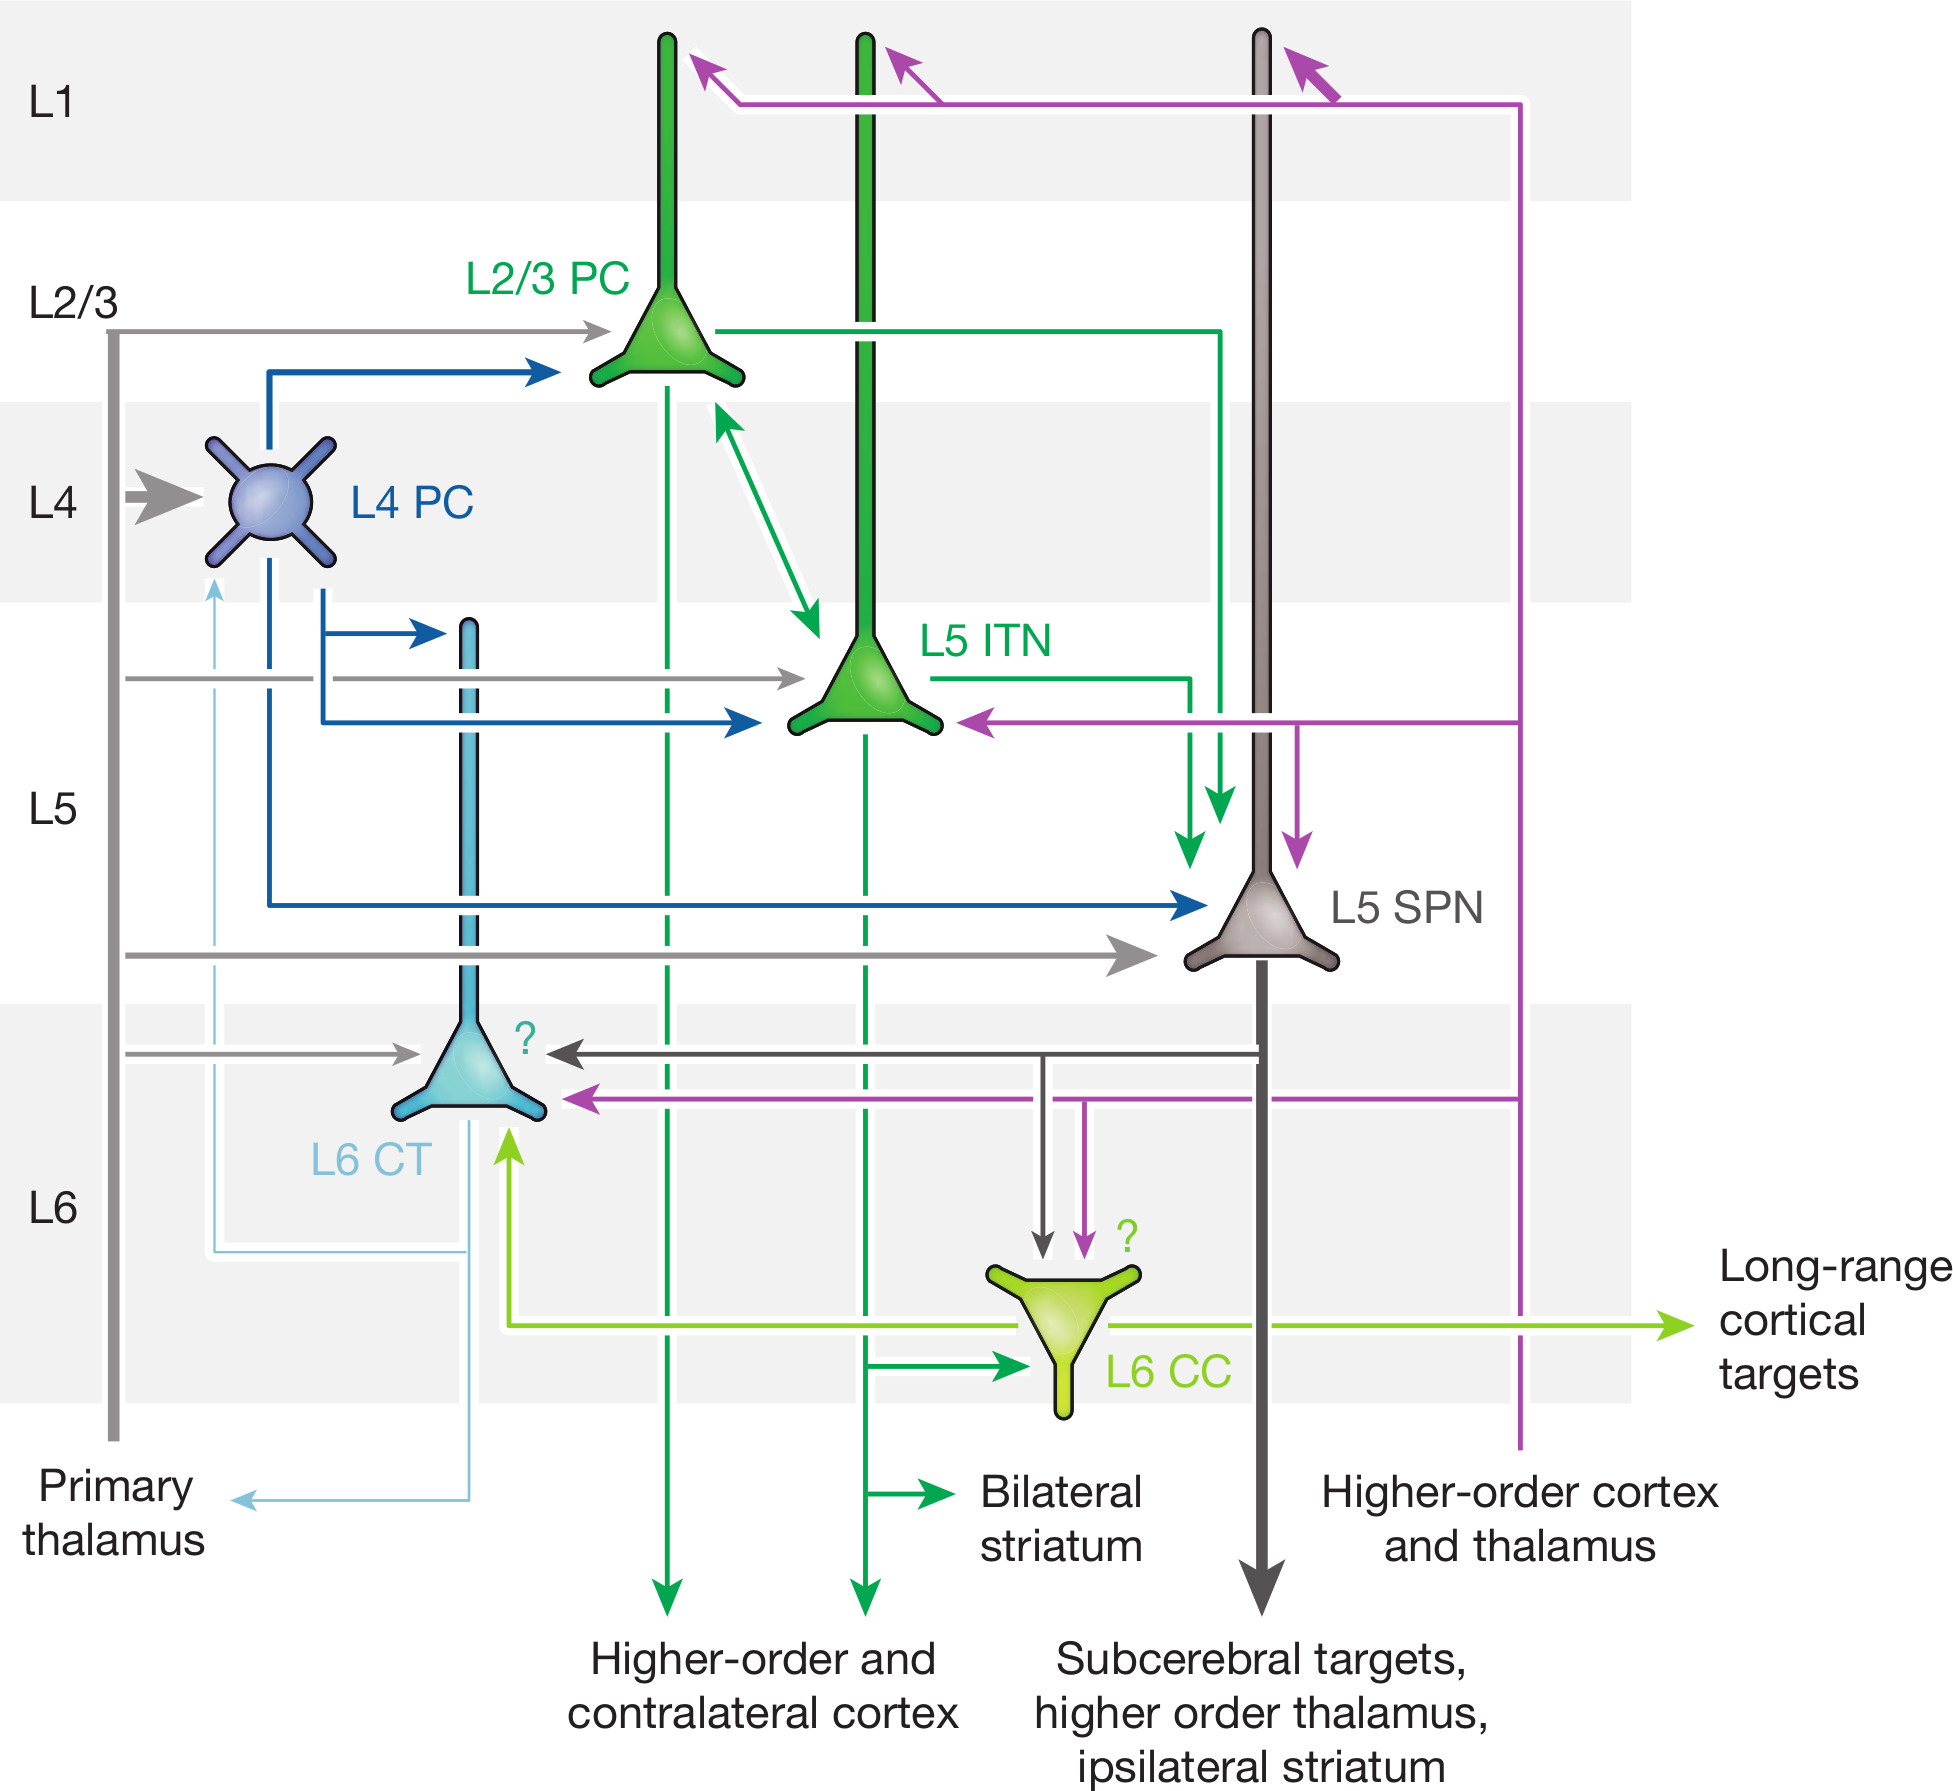
\includegraphics[width=\linewidth]{postdiss/cortconn.jpg}

\caption{\justifying\scriptsize Canonical connectivity of cortical principal 
cells~\cite{Kerdels2018}.}
\end{figure}

}

\vspace{-0.5em}

\begin{center}
\rule{2cm}{0.4pt}\\[0.5em]
\end{center}

\fc{Kerdels2018}{publications/2018-01/2018-01}\\[1em]
\fc{Kerdels2019b}{publications/2019-03/2019-03}

\end{frame}


\begin{frame}{Towards a Model of Cortical Function \sof{2}{2}}

\vspace{0.5em}
\justifying
In~\cite{Kerdels2020} we revisit the algorithm underlying our grid cell model
and present an {\bf efficient approximation} of the original algorithm that is 
more robust regarding the formation of the group’s input space representation, 
is structurally less complex, and is computationally more efficient.

\vspace{1em}

\begin{figure}
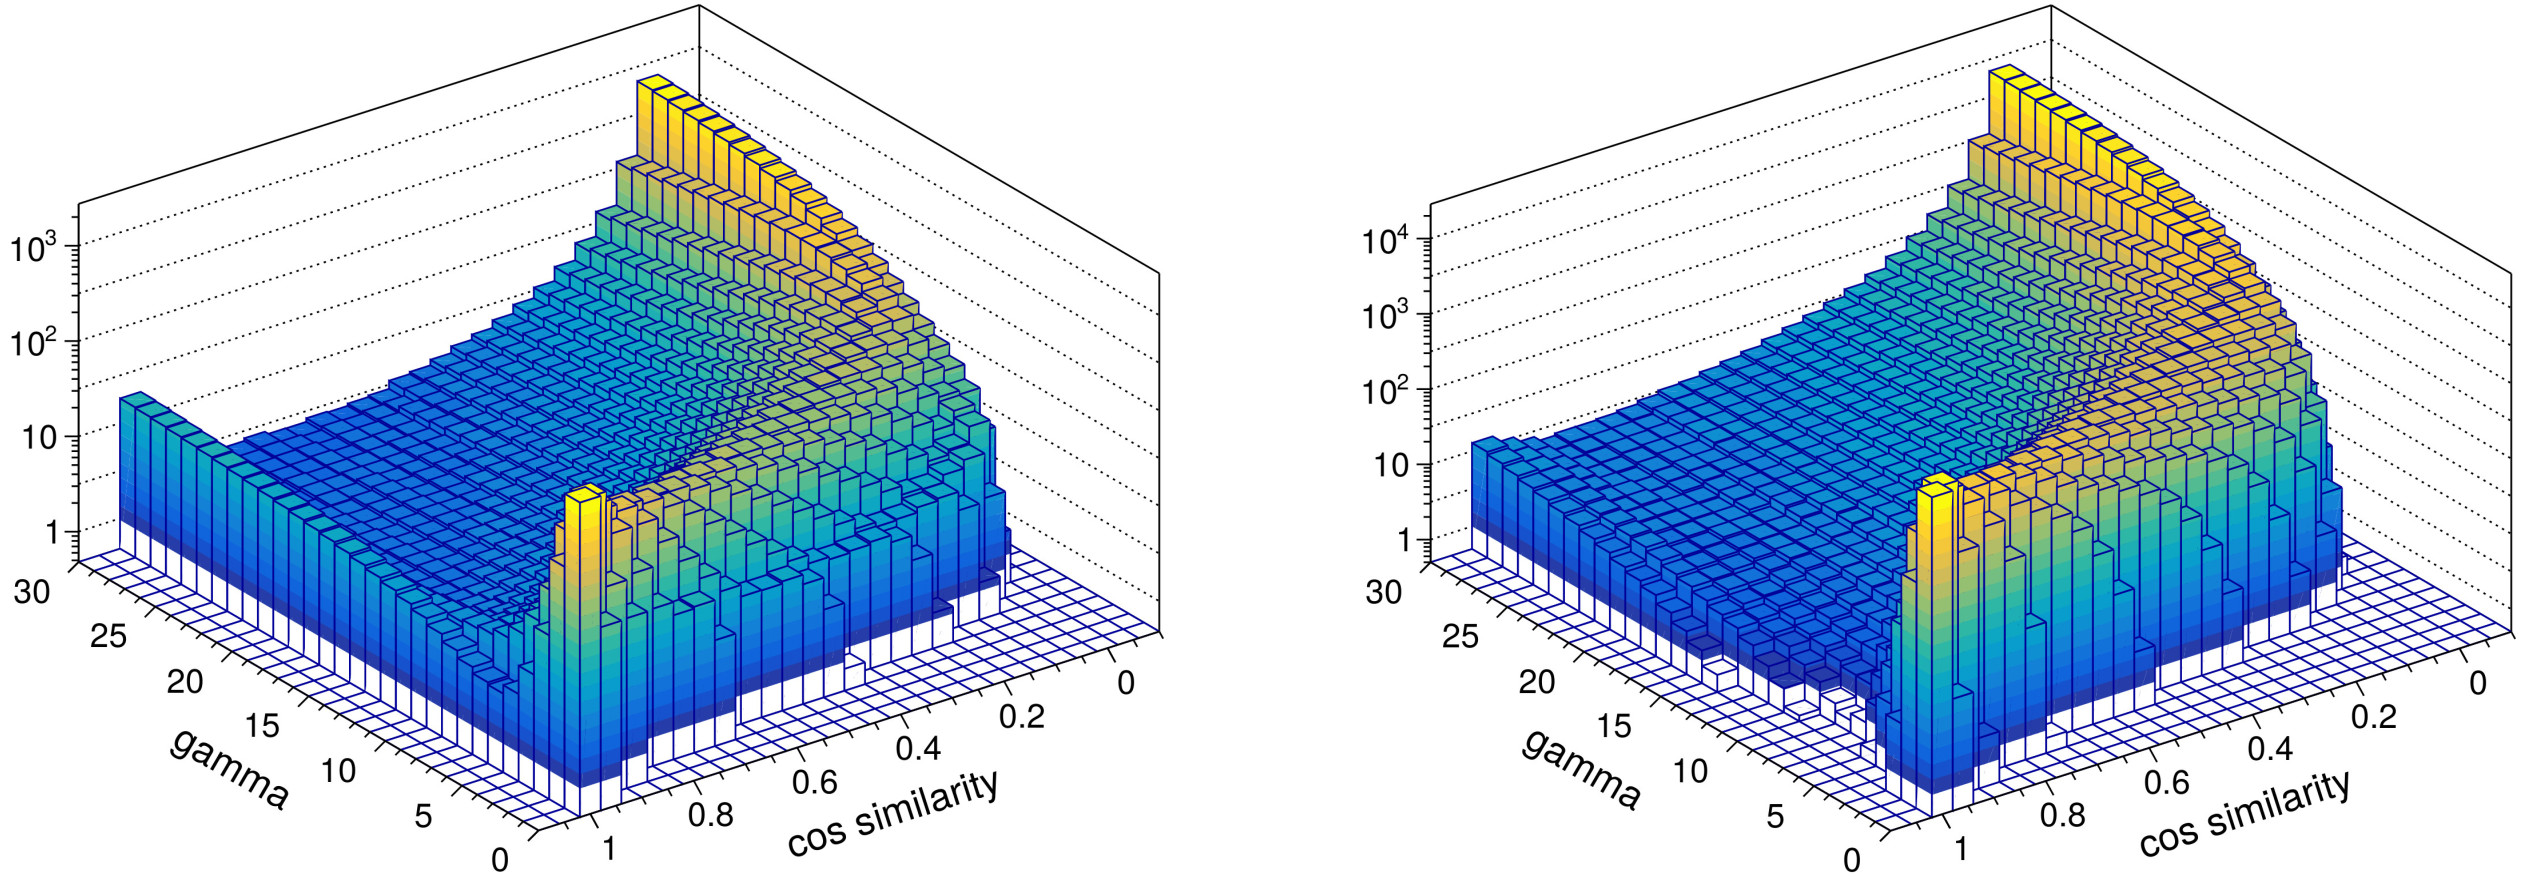
\includegraphics[width=0.8\linewidth]{postdiss/patsep.jpg}

\caption{\justifying\scriptsize Histograms of pairwise cosine similarities 
between ensemble activity vectors of a modeled neuron group in response to the 
MNIST test dataset. Left shows cosine similarities for intra-class samples. 
Right shows the results for inter-class samples. Details in~\cite{Kerdels2020}.}
\end{figure}

\begin{center}
\rule{2cm}{0.4pt}\\[0.5em]
\end{center}

\fc{Kerdels2020}{publications/2020-01/2020-01}

\end{frame}



